\documentclass[a4paper]{article}
\usepackage{tikz}
%\usepackage{algorithm}[boxed]
\usepackage{algorithmic}
\usetikzlibrary{petri,automata,matrix,backgrounds,arrows}

\title{Creating a single safe conservative Petri Net from multiple DFAs}
\author{Andrew Matthews}
\date{\today}
\begin{document}
\maketitle
\begin{abstract}
Telephony, like many other industrial applications of Finite Automata, often utilizes numerous orthogonal state machines to represent independent aspects of the problem and solution domain to remain comprehensible to a business audience. Such an approach introduces potential flaws into a system by increasing the state space to illegal combinations. There are various ways to try to restrict the model to 'valid' state combinations. This paper explores one solution that combines the state models into a single extended generalized Petri Net whilst staying safe, live, bounded and conservative. The model presented is globally bounded, but is locally unbounded. By losening the restrictions normally imposed on petri nets directly translated from state models we are able to demonstrate control between state models that is not possible using orthogonal state machines.
\end{abstract}

\section{Introduction}
In many problem domains, and particularly in telephony, it is nec essary to model the problem domain using several orthogonal DFAs. This approach makes the model easier to comprehend for a non-specialist audience and makes it easier to predict the effects of state model changes to system behaviour. 

In the system my team has been working on are over a dozen orthogonal state machines. The approach of using such concurrent state models has been extremely successful, allowing domain experts to contribute to the modelling of the system and providing a meaningful extensibility model for the rest of the software to hang off. 

With the unification of messaging and telephony platforms we saw the number of state models increase continually. Trying to integrate new features into a monolithic state model would very quickly have become impossible. Factorising the state models allowed the introduction of new systems without significant extra effort. This extensibility and maintainability came at a cost. This paper arose out of an effort to address the potential for state 'corruption' implicit in the factorised state model.

In distributed event driven systems with unreliable messaging channels, it is entirely possible -- in fact it is probable -- that the system will leave the 'correct' state space and transition into spaces that while strictly legal are in actuality wrong. Normally, the result of that happening is a loss of call control for the user. We have previously addressed such flaws by utilizing heuristic knowledge about permissible states and rectifying deviations by controlling the state model directly. Clearly, such a model is less desirable than one that disallows undesirable states.

\section{Potential solutions}
Consider two state models, $SM_1$ and $SM_2$, like so

\begin{figure}[ht]
	\begin{center}
		\begin{tikzpicture} [background rectangle/.style={fill=yellow!20}, framed,show
			background rectangle,yscale=1.5,thin,>=stealth,thick,
			every transition/.style={fill,minimum width=1mm,minimum height=7mm},
			original state/.style={blue!50!black!50,top color=white,bottom color=blue!20},
			input state/.style={red!50!black!50,top color=white,bottom color=red!20},
			control state/.style={green!50!black!50,top color=white,bottom color=green!20},
			every place/.style={draw,very thick,minimum size=6mm},
			inhibitor/.style={o-},
			exhaust/.style={red!70!black!70!,top color=red!20,bottom color=red}
			]

\end{tikzpicture}\end{center}\end{figure}


\begin{figure}[ht]
	\begin{center}
		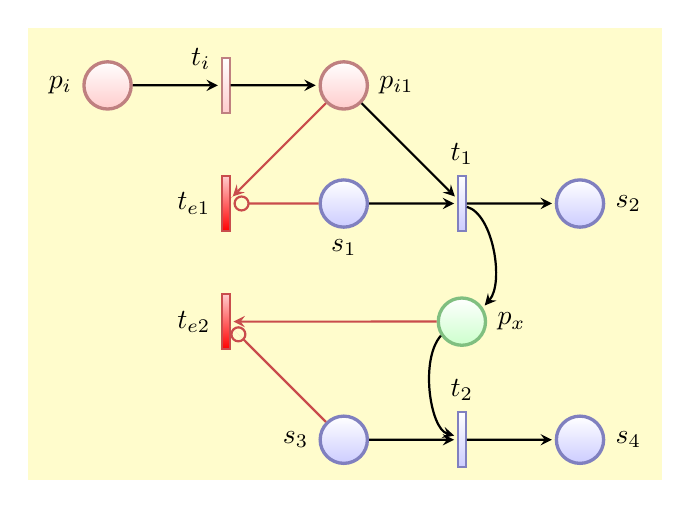
\begin{tikzpicture} [background rectangle/.style={fill=yellow!20}, framed,show
			background rectangle,yscale=1.5,thin,>=stealth,thick,
			every transition/.style={fill,minimum width=1mm,minimum height=7mm},
			original state/.style={blue!50!black!50,top color=white,bottom color=blue!20},
			input state/.style={red!50!black!50,top color=white,bottom color=red!20},
			control state/.style={green!50!black!50,top color=white,bottom color=green!20},
			every place/.style={draw,very thick,minimum size=6mm},
			inhibitor/.style={o-},
			exhaust/.style={red!70!black!70!,top color=red!20,bottom color=red}
			]
		%\draw[step=1cm, color=gray] (-1, -1) grid (10,5);
		\node [place, original state, label=below:$s_1$] (p1) at (2.5,3) {};
		\node [place, input state, label=right:$p_{i1}$] (pi1) at (2.5,4) {};
		\node [place, original state, label=right:$s_2$] (p2) at (5.5,3) {};
		\node [place, input state, label=left:$p_i$] (pi) at (-0.5,4) {};
		\node [place, control state, label=right:$p_{x}$] (px) at (4,2) {};
		\node [place, original state, label=left:$s_3$] (p3) at (2.5,1) {};
		\node [place, original state, label=right:$s_4$] (p4) at (5.5,1) {};

		\node [transition, original state, label=above:$t_1$] (t1) at (4,3) {}
			edge [pre] (p1)
			edge [pre] (pi1)
			edge [post, bend left=66] (px)
			edge [post] (p2);
		\node [transition, original state, label=above:$t_2$] (t2) at (4,1) {}
			edge [pre] (p3)
			edge [pre, bend left=66] (px)
			edge [post] (p4);

		\node [transition, exhaust, label=left:$t_{e1}$] (te1) at (1,3) {}
			edge [pre, exhaust, inhibitor] (p1) %inhibitor
			edge [pre, exhaust] (pi1);

		\node [transition, exhaust, label=left:$t_{e2}$] (te2) at (1,2) {}
			edge [pre, exhaust, inhibitor] (p3) %inhibitor
			edge [pre, exhaust] (px);

		\node [transition, input state, label=above left:$t_i$] (ti) at (1,4) {}
			edge [pre] (pi)
			edge [post] (pi1);
		\end{tikzpicture}
	\end{center}
	\caption{A petri net that reproduces the semantics of Fig. \ref{fig:dfa1} while
	consuming unused tokens}
	\label{fig:ptnetfinal}
\end{figure}

\begin{figure}[ht]
	\begin{center}
		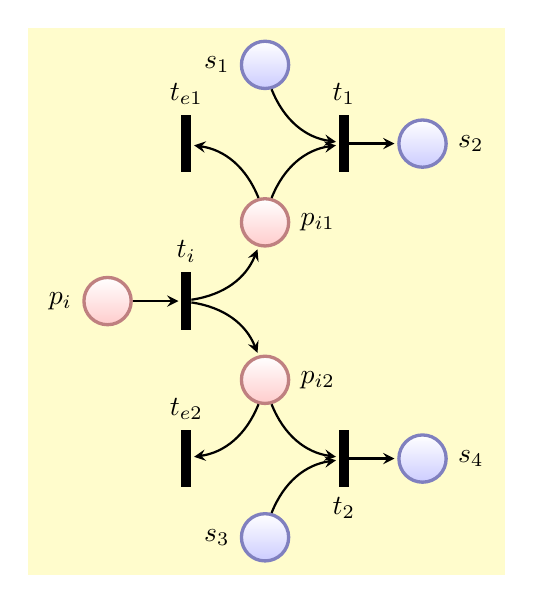
\begin{tikzpicture} [background rectangle/.style={fill=yellow!20}, framed,show
			background rectangle,yscale=1,thin,>=stealth,thick,
			every transition/.style={fill,minimum width=1mm,minimum height=7mm},
			original state/.style={blue!50!black!50,top color=white,bottom color=blue!20},
			input state/.style={red!50!black!50,top color=white,bottom color=red!20},
			every place/.style={draw,very thick,minimum size=6mm}
			]

		\node [place, original state, label=left:$s_1$] (s1) at (3,7) {};
		\node [place, input state, label=right:$p_{i1}$] (pi1) at (3,5) {};
		\node [place, original state, label=right:$s_2$] (s2) at (5,6) {};
		\node [place, input state, label=left:$p_i$] (pi) at (1,4) {};
		\node [place, input state, label=right:$p_{i2}$] (pi2) at (3,3) {};
		\node [place, original state, label=left:$s_3$] (s3) at (3,1) {};
		\node [place, original state, label=right:$s_4$] (s4) at (5,2) {};

		\node [transition, label=above:$t_{e1}$] (te1) at (2,6) {}
			edge [pre, bend left] (pi1);
		\node [transition, label=above:$t_1$] (t1) at (4,6) {}
			edge [pre, bend left] (s1)
			edge [pre, bend right] (pi1)
			edge [post] (s2);
		\node [transition, label=above:$t_i$] (ti) at (2,4) {}
			edge [pre] (pi)
			edge [post, bend right] (pi1)
			edge [post, bend left] (pi2);
		\node [transition, label=above:$t_{e2}$] (te2) at (2,2) {}
			edge [pre, bend right] (pi2);
		\node [transition, label=below:$t_2$] (t2) at (4,2) {}
			edge [pre, bend right] (s3)
			edge [pre, bend left] (pi2)
			edge [post] (s4);

		\end{tikzpicture}
	\end{center}
	\caption{A petri net that reproduces the semantics of Fig. \ref{fig:dfa1} while
	consuming unused tokens}
	\label{fig:ptnetfinal}
\end{figure}


\section{Introduction}
% state the problem 
% give some examples of where the problem arises
% give examples of how illegal state combinations arise

\section{Academic-style State Machine Petri Nets}
% standard definitions of state model petri nets
% flaws in this model
% simple solutions
\subsection{Factorising a state space using a naive petri net}
% flaws in the simple solution
%	no solution to factorising the state space - i.e. 1-1 still allows
%		illegal combinations
%	adding arcs between factorised state spaces is not conservative
\section{Input places}
% A less naive solution - using places for  state transition inputs
%	Hanging tokens in input places
%	using exhaust transitions
%	controlling firing priority
%	state predication or inhibition is not conservative or safe
\end{document}



